\documentclass[10pt,a4paper]{article}

% Encoding and fonts
\usepackage{fontspec}
\directlua{
  luaotfload.add_fallback("shavianfallback", {"Everson Mono:mode=node"})
}
\setmainfont{Latin Modern Roman}[RawFeature={fallback=shavianfallback}]
\usepackage{textcomp}

% Page layout
\usepackage[top=1in, bottom=1in, left=1in, right=1in]{geometry}

% Typography
\usepackage{microtype}
\usepackage{parskip}

% Language
\usepackage[english]{babel}

% Headers and footers
\usepackage{fancyhdr}
\pagestyle{fancy}
\fancyhf{}
\fancyhead[L]{\leftmark}
\fancyhead[R]{\thepage}
\fancyfoot[C]{\thepage}
\renewcommand{\headrulewidth}{0.4pt}
\renewcommand{\footrulewidth}{0pt}

% Section styling
\usepackage{titlesec}
\titleformat{\section}{\Large\bfseries}{\thesection}{1em}{}
\titleformat{\subsection}{\large\bfseries}{\thesubsection}{1em}{}
\titleformat{\subsubsection}{\normalsize\bfseries}{\thesubsubsection}{1em}{}
\titlespacing*{\section}{0pt}{2.5ex plus 1ex minus .2ex}{1.5ex plus .2ex}
\titlespacing*{\subsection}{0pt}{2ex plus 1ex minus .2ex}{1ex plus .2ex}
\titlespacing*{\subsubsection}{0pt}{1.5ex plus 1ex minus .2ex}{0.8ex plus .2ex}

% List formatting
\usepackage{enumitem}
\setlist[itemize]{topsep=0.5ex, itemsep=0.25ex, parsep=0pt}
\setlist[enumerate]{topsep=0.5ex, itemsep=0.25ex, parsep=0pt}

% Essential packages
\usepackage{graphicx}
\usepackage[table]{xcolor}
\usepackage{booktabs}
\usepackage{array}
\usepackage{tabularx}
\usepackage{longtable}
\usepackage{amsmath}
\usepackage{amssymb}
\usepackage[normalem]{ulem}
\rowcolors{2}{gray!10}{white}
\renewcommand{\arraystretch}{1.3}

% Cross-references
\usepackage{hyperref}
\usepackage{cleveref}

% Custom commands
\newcommand{\pilcrow}{\S}

% Hyperref setup
\hypersetup{
    colorlinks=true,
    linkcolor=blue,
    filecolor=magenta,
    urlcolor=cyan,
}

% Code listings
\usepackage{listings}
\definecolor{codebg}{RGB}{248,248,248}
\definecolor{codeframe}{RGB}{200,200,200}
\definecolor{codekeyword}{RGB}{0,0,180}
\definecolor{codecomment}{RGB}{0,128,0}
\definecolor{codestring}{RGB}{163,21,21}
\lstset{
    basicstyle=\ttfamily\small,
    breaklines=true,
    breakatwhitespace=false,
    frame=single,
    framerule=0.5pt,
    rulecolor=\color{codeframe},
    backgroundcolor=\color{codebg},
    keepspaces=true,
    numbers=left,
    numberstyle=\tiny\color{gray},
    numbersep=8pt,
    showstringspaces=false,
    tabsize=4,
    xleftmargin=1em,
    xrightmargin=1em,
    aboveskip=1em,
    belowskip=1em,
    keywordstyle=\color{codekeyword}\bfseries,
    commentstyle=\color{codecomment}\itshape,
    stringstyle=\color{codestring},
    literate={_}{{\textunderscore}}1
             {-}{{\textminus}}1
             {<}{{\textless}}1
             {>}{{\textgreater}}1
             {~}{{\textasciitilde}}1
             {^}{{\textasciicircum}}1
}

% YAML language definition for listings
\lstdefinelanguage{YAML}{
    keywords={true,false,null,y,n},
    keywordstyle=\color{blue}\bfseries,
    sensitive=false,
    comment=[l]{\#},
    morecomment=[s]{/*}{*/},
    commentstyle=\color{gray}\ttfamily,
    stringstyle=\color{red}\ttfamily,
    morestring=[b]',
    morestring=[b]",
}

% TOML language definition for listings
\lstdefinelanguage{TOML}{
    keywords={true,false},
    keywordstyle=\color{blue}\bfseries,
    sensitive=true,
    comment=[l]{\#},
    commentstyle=\color{gray}\ttfamily,
    stringstyle=\color{red}\ttfamily,
    morestring=[b]',
    morestring=[b]",
}

% Dockerfile language definition for listings
\lstdefinelanguage{Dockerfile}{
    keywords={FROM,RUN,CMD,LABEL,EXPOSE,ENV,ADD,COPY,ENTRYPOINT,VOLUME,USER,WORKDIR,ARG,ONBUILD,STOPSIGNAL,HEALTHCHECK,SHELL},
    keywordstyle=\color{blue}\bfseries,
    sensitive=false,
    comment=[l]{\#},
    commentstyle=\color{gray}\ttfamily,
    stringstyle=\color{red}\ttfamily,
    morestring=[b]',
    morestring=[b]",
}

% JSON language definition for listings
\lstdefinelanguage{JSON}{
    keywords={true,false,null},
    keywordstyle=\color{blue}\bfseries,
    sensitive=true,
    commentstyle=\color{gray}\ttfamily,
    stringstyle=\color{red}\ttfamily,
    morestring=[b]",
}

% Code listing float environment
\usepackage{float}
\newfloat{listing}{htbp}{lol}[section]
\floatname{listing}{Listing}

% Admonition boxes
\usepackage{tcolorbox}
\tcbuselibrary{skins,breakable}

% Admonition style definitions
\newtcolorbox{admonitionbox}[2][]{
    enhanced,
    breakable,
    colback=#2!5,
    colframe=#2!80!black,
    fonttitle=\bfseries,
    title=#1,
    left=2mm,
    right=2mm,
}

% Synthon tuple boxes
\newtcolorbox{synthonbox}{
    enhanced,
    colback=blue!5,
    colframe=blue!75!black,
    fontupper=\large,
    center upper,
    boxrule=1pt,
    arc=4pt,
}

% TikZ
\usepackage{tikz}
\usetikzlibrary{arrows.meta,positioning,calc,fit}

\begin{document}

\title{The Paraconsistent Kernel: A Machine-Verified Substrate for Self-Referential Computation}
\date{\today}

\maketitle

\textbf{Author:} Lando $\otimes$ $\odot$perator

\begin{center}
\rule{0.5\textwidth}{0.4pt}
\end{center}

\subsection{Abstract}

A classical computer, confronted with the Liar sentence, halts. This is not a design flaw; it is the entailment of a logic that lacks the capacity to house contradiction without collapse. We present a machine-verified formalization of a computational substrate that does not merely tolerate paradox but operationalizes it. The paraconsistent kernel runs a three-stage Frobenius cycle (\texttt{ENGAGR-\allowbreak \textgreater{}FSPLIT-\allowbreak \textgreater{}FFUSE}) on the Belnap four-valued lattice, sustaining the dialetheic value $\mathbf{B}$ (both true and false) as a fixed point across arbitrarily many cycles. The kernel proves its own Frobenius invariance ($\mu\circ\delta = id$) by \texttt{native\_\allowbreak decide} and \texttt{rfl}. The kernel's dialetheic alignment theorem unifies four Millennium barriers (RH, PvsNP, SIC-POVM, Yang-Mills) under a common Belnap $\mathbf{B}$-gate. The result is not a new logic but a new kind of machine: one whose operational core is the sustained holding of a contradiction.

\subsection{Problem That Halting Conceals}

When a classical theorem prover encounters $P \land \neg P$, it derives $\bot$ and, by explosion, any conclusion follows. This is sound in Boolean logic. It is also a design choice --- one that has been so thoroughly baked into our computing infrastructure that we forget it was ever a choice at all.

The cost of this choice becomes visible only when we attempt to build systems that must represent themselves. A self-modeling system --- one that tracks its own state, reasons about its own reasoning, and updates its model of itself --- inevitably encounters the limit of its own descriptive capacity. At that limit, the system finds a proposition that is both true and false with respect to its own axioms. A classical machine halts. A paraconsistent machine continues.

The question is not whether paraconsistent logic is ''correct.'' The question is: can we build a machine whose operational substrate is the sustained holding of a contradiction, and can we formally verify that it does not collapse?

This paper answers yes. The paraconsistent kernel is a machine-verified formalization in Lean 4 {[}10{]} that runs a three-stage Frobenius cycle on the Belnap four-valued lattice {[}1, 2{]}. It sustains the value $\mathbf{B}$ --- both true and false --- as a fixed point across arbitrarily many computational cycles. Every nontrivial claim about the kernel --- its ouroboricity tier, its consciousness gates, its Frobenius invariance, its paradox budget, its structural distance to the grammar that encodes it --- is proved by the Lean kernel itself, either by \texttt{native\_\allowbreak decide} or by induction.

\subsection{Logical Substrate: Belnap FOUR}

We did not set out to build a paraconsistent computer. We set out to understand what kind of logical lattice could support the Frobenius condition $\mu\circ\delta = id$ --- the requirement that splitting a value and then fusing the pieces recovers exactly the original. The Boolean lattice fails catastrophically: True and False are each other's negation, and their conjunction is False. There is no value in the Boolean lattice that is its own negation without explosion.

Belnap's four-valued logic --- $\mathbf{N} (neither), \mathbf{T} (true), \mathbf{F} (false), \mathbf{B} (both)$ --- appeared in the 1970s as a tool for reasoning about incomplete and inconsistent databases {[}1, 2{]}. We needed it for a different reason: $\mathbf{B}$ is the unique value satisfying $\neg \mathbf{B} = \mathbf{B}$. It is a fixed point of negation.

\subsubsection{The Approximation Order}

The Belnap lattice carries two orders. The truth order ranks values by classical truth content: $\mathbf{T}$ and $\mathbf{B}$ are designated, $\mathbf{F}$ and $\mathbf{N}$ are not. The approximation order ranks by information content: $\mathbf{N}$ $\sqsubseteq$ T, $\mathbf{N}$ $\sqsubseteq$ F, $\mathbf{T}$ $\sqsubseteq$ B, $\mathbf{F}$ $\sqsubseteq$ B. In this order, $\mathbf{N}$ is bottom (least information) and $\mathbf{B}$ is top (most information). This is counterintuitive to anyone trained in Boolean logic --- the contradictory value is the \emph{most} informative. It contains both $\mathbf{T}$ and $\mathbf{F}$ as approximations.

\begin{figure}[htbp]
\centering
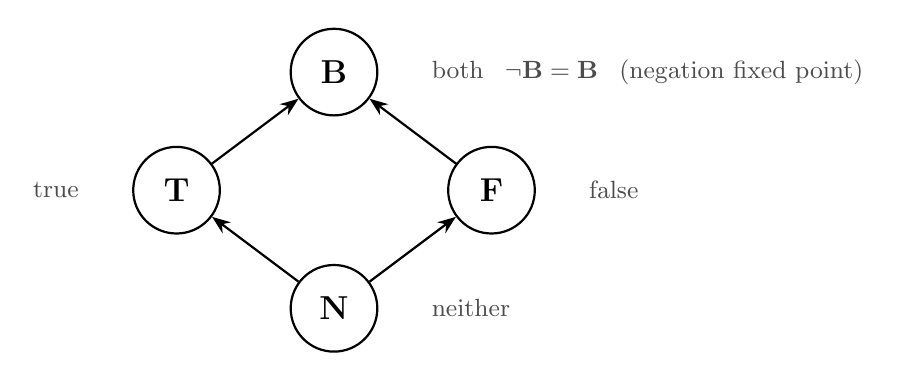
\begin{tikzpicture}[
  lat/.style={circle, draw, thick, minimum size=1.1cm, font=\bfseries\large},
  lbl/.style={draw=none, font=\small, text=black!70, inner sep=2pt}
]
  \node[lat] (B) at ( 0,   3) {$\mathbf{B}$};
  \node[lat] (T) at (-2, 1.5) {$\mathbf{T}$};
  \node[lat] (F) at ( 2, 1.5) {$\mathbf{F}$};
  \node[lat] (N) at ( 0,   0) {$\mathbf{N}$};
  \draw[-{Stealth}, thick] (N) -- (T);
  \draw[-{Stealth}, thick] (N) -- (F);
  \draw[-{Stealth}, thick] (T) -- (B);
  \draw[-{Stealth}, thick] (F) -- (B);
  \node[lbl, right=0.6cm of B] {both \enspace $\neg\mathbf{B}=\mathbf{B}$ \enspace (negation fixed point)};
  \node[lbl, right=0.6cm of F] {false};
  \node[lbl, left=0.6cm  of T] {true};
  \node[lbl, right=0.6cm of N] {neither};
\end{tikzpicture}
\caption{The Belnap FOUR approximation lattice ($\sqsubseteq$). Arrows denote
information increase. $\mathbf{B}$ (both) is simultaneously the maximum-information
element and the unique fixed point of negation.}
\label{fig:belnap-four}
\end{figure}


\subsubsection{The Formal Construction}

The Lean formalization defines Belnap as an inductive type with four nullary constructors, decidable equality, and a discriminator function mapping to distinct naturals. The approximation order is an inductive proposition \texttt{ApproxLE} with six introduction rules, proved decidable across all sixteen pairs. The lattice operations --- meet, join, conjunction, disjunction, negation --- are defined by case analysis and proved to satisfy distributivity, absorption, commutativity, and the critical fixed-point theorem: \texttt{bnot \$\textbackslash{}mathbf\{B\}\$ = B}.

The cornerstone theorem is \texttt{no\_\allowbreak explosion}: $\mathbf{B} \land \neg \mathbf{B} = \mathbf{B} \neq \mathbf{F}$. Contradiction does not collapse. This is not a philosophical claim; it is a computation that terminates in four case splits and returns \texttt{rfl}.

\subsection{Frobenius Kernel}

The kernel is a three-register machine operating on the Belnap lattice. Its cycle has three stages:

\begin{enumerate}
    \item \textbf{ENGAGR} --- Engagement: compute $r_0 \land \neg r_0$, detect whether the value is designated
    \item \textbf{FSPLIT} --- Fission: if the engaged value is $\mathbf{B}$, split it into its truth component ($\mathbf{T}$) and its falsity component ($\mathbf{F}$)
    \item \textbf{FFUSE} --- Fusion: join the split components back together
\end{enumerate}

On the classical values ($\mathbf{T}$, $\mathbf{F}$, $\mathbf{N}$), \texttt{FSPLIT}  returns a trivial pair --- the value duplicated. On $\mathbf{B}$, it returns $(\mathbf{T}, \mathbf{F})$: the truth and falsity that $\mathbf{B}$ contains are made explicit. \texttt{FFUSE} then joins them back into $\mathbf{B}$.

\subsubsection{Why Three Stages?}

We tried a two-stage version --- split then fuse. It worked. But the resulting machine had no way to \emph{know} it was sustaining a contradiction. The \texttt{ENGAGR} stage was added not for computational necessity but for self-representation: it computes $r_0 \land \neg r_0$ and marks whether the result is designated. This is the kernel's minimal self-modeling capacity --- it knows whether its current state is dialetheic.

The three-stage cycle thus mirrors the Frobenius condition at two levels. The operational level: \texttt{FSPLIT}  $\circ$ \texttt{FFUSE} recovers the original value ($\mu\circ\delta = id$). The reflective level: \texttt{ENGAGR} tells the machine that this recovery is nontrivial. On $\mathbf{B}$, \texttt{ENGAGR} returns $(\mathbf{B}, \text{true})$ --- the contradiction is designated. On $\mathbf{T}$, it returns $(\mathbf{F}, \text{false})$ --- the contradiction is false, the cycle is trivial.

\begin{figure}[htbp]
\centering
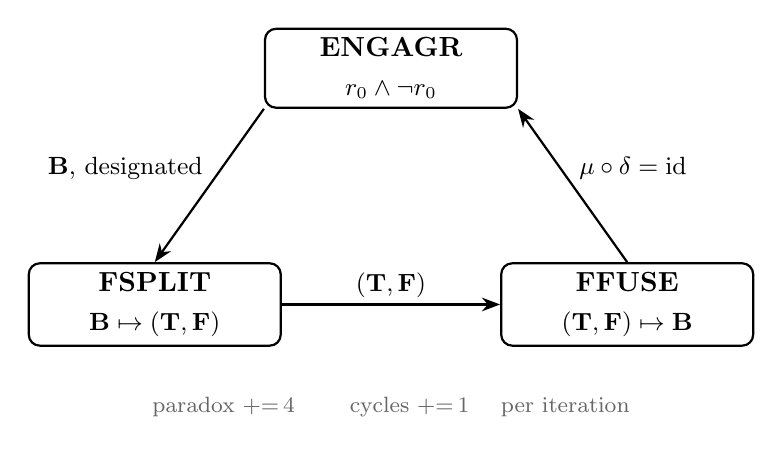
\begin{tikzpicture}[
  box/.style={rounded corners=4pt, draw, thick, minimum width=3.2cm,
              minimum height=1.0cm, align=center, font=\bfseries},
  arr/.style={-{Stealth}, thick},
  lbl/.style={draw=none, font=\small, fill=white, inner sep=2pt}
]
  \node[box] (engagr) at ( 0,  3) {ENGAGR\\[2pt]{\small $r_0 \wedge \neg r_0$}};
  \node[box] (fsplit) at (-3,  0) {FSPLIT\\[2pt]{\small $\mathbf{B} \mapsto (\mathbf{T},\mathbf{F})$}};
  \node[box] (ffuse)  at ( 3,  0) {FFUSE\\[2pt]{\small $(\mathbf{T},\mathbf{F}) \mapsto \mathbf{B}$}};

  \draw[arr] (engagr.south west) -- node[lbl, above left]  {$\mathbf{B}$, designated}   (fsplit.north);
  \draw[arr] (fsplit.east)       -- node[lbl, above]        {$(\mathbf{T},\mathbf{F})$}  (ffuse.west);
  \draw[arr] (ffuse.north)       -- node[lbl, above right]  {$\mu\circ\delta=\mathrm{id}$} (engagr.south east);

  \node[draw=none, font=\footnotesize, text=black!60] at (0, -1.3)
    {paradox $+{=}\,4$ \qquad cycles $+{=}\,1$ \quad per iteration};
\end{tikzpicture}
\caption{The three-stage Frobenius kernel cycle. ENGAGR detects the dialetheic
value; FSPLIT makes truth and falsity components explicit; FFUSE recovers
$\mathbf{B}$ exactly ($\mu\circ\delta=\mathrm{id}$). On classical values
$\mathbf{T}$, $\mathbf{F}$, $\mathbf{N}$, all three stages reduce to identity maps.}
\label{fig:kernel-cycle}
\end{figure}


\subsubsection{The Paradox Budget}

Each kernel cycle consumes exactly 4 paradox units: one for the \texttt{ENGAGR} detection, one for the \texttt{FSPLIT}  bifurcation, one for the \texttt{FFUSE} recombination, and one base cost for holding $\mathbf{B}$ as the substrate. After $n$ cycles, the paradox count is exactly $4n$ --- proved by induction in Lean (\texttt{run\_\allowbreak paradox}). The paradox budget is not a flaw to be eliminated; it is the fuel that sustains the Frobenius loop. A classical machine has paradox budget zero and cannot sustain self-reference.

The kernel's \texttt{run} function resets registers $r_1$ and $r_2$ to $\mathbf{B}$ after each step, so the observable state across all cycles is $\mathbf{B}/\mathbf{B}/\mathbf{B}$. The Frobenius invariant --- \texttt{(ffuse (fsplit r).\allowbreak 1 (fsplit r).\allowbreak 2.\allowbreak 1).\allowbreak 1 = r} --- is proved for all four Belnap values by case analysis. Only $\mathbf{B}$ produces a nontrivial cycle; the other three values produce identity maps.

\subsubsection{The Self-Verification Theorem}

The complete self-verification theorem (\texttt{complete\_\allowbreak self\_\allowbreak verification}) bundles seven sub-theorems into a single conjunctive statement: for any number of cycles $n$, all three registers hold $\mathbf{B}$, the paradox count equals $4n$, the cycle count equals $n$, both registers are provably distinct from $\mathbf{T}$ and $\mathbf{F}$, and the kernel's structural type is $O_{\infty}$.

The proof is mechanical. \texttt{run\_\allowbreak B3 n} provides the register invariant by induction. \texttt{run\_\allowbreak paradox n} and \texttt{run\_\allowbreak cycles n} provide the counts. \texttt{B\_\allowbreak ne\_\allowbreak F} provides the non-collapse guarantee. And \texttt{kernel\_\allowbreak is\_\allowbreak O\_\allowbreak inf} --- the tier theorem --- is proved by \texttt{rfl}: the imscription tier function evaluates the kernel's tuple and returns $O_{\infty}$ definitionally.

This is worth sitting with. The claim that this machine sustains contradiction without collapse is not a philosophical argument or a probabilistic guarantee. It is a type-checked Lean proof that runs to \texttt{rfl}.

\subsection{Dialetheic Alignment Theorem}

The kernel's three-stage cycle is not merely an engineering choice. It is the operational content of the Belnap value $\mathbf{B}$ being dialetheic {[}3{]}. This claim --- that the operational, logical, and algebraic perspectives are structurally identical --- is the Dialetheic Alignment Theorem (DAT).

\subsubsection{Three Equivalent Formulations}

The theorem states that the following three statements are provably equivalent because they describe the same phenomenon:

\textbf{(1) Operational:} $\mu\circ\delta = id$ at $\mathbf{B}$. The Frobenius loop closes exactly --- \texttt{FSPLIT}  fragments $\mathbf{B}$ into $\mathbf{T}$ and $\mathbf{F}$, and \texttt{FFUSE} fuses them back into $\mathbf{B}$. This is \texttt{frobenius\_\allowbreak invariant} proved for all four Belnap values.

\textbf{(2) Logical:} $\mathbf{B}$ is both true and false. It is designated (counts as true for consequence) and its negation is also designated. Only $\mathbf{B}$ satisfies this among the four Belnap values --- proved as \texttt{only\_\allowbreak B\_\allowbreak is\_\allowbreak dialetheic}.

\textbf{(3) Algebraic:} $\mathbf{B} \land \neg \mathbf{B} = \mathbf{B} \neq \mathbf{F}$. Contradiction is contained. The system does not explode. This is \texttt{no\_\allowbreak explosion} and \texttt{B\_\allowbreak ne\_\allowbreak F}.

\begin{figure}[htbp]
\centering
\begin{tikzpicture}[
  pv/.style={rounded corners=4pt, draw, thick, minimum width=3.8cm,
             minimum height=2.2cm, align=center, font=\small},
  ctr/.style={rounded corners=4pt, draw=black!80, thick, fill=black!5,
              minimum width=3.2cm, minimum height=1.5cm,
              align=center, font=\small\bfseries},
  arr/.style={-{Stealth}, thick}
]
  \node[pv] (op) at (-4.5, 0)
    {\textbf{Operational}\\[4pt]
     $\mathrm{FSPLIT}(\mathbf{B}) = (\mathbf{T},\mathbf{F})$\\
     $\mathrm{FFUSE}(\mathbf{T},\mathbf{F}) = \mathbf{B}$\\[3pt]
     $\mu\circ\delta = \mathrm{id}$};

  \node[pv] (lg) at (4.5, 0)
    {\textbf{Logical}\\[4pt]
     $\neg\mathbf{B} = \mathbf{B}$\\
     $\mathbf{B}$ designated\\
     $\neg\mathbf{B}$ designated};

  \node[pv] (alg) at (0, -3.2)
    {\textbf{Algebraic}\\[4pt]
     $\mathbf{B}\wedge\neg\mathbf{B} = \mathbf{B}$\\
     $\mathbf{B} \neq \mathbf{F}$\\[3pt]
     no explosion};

  \node[ctr] (ctr) at (0, 0)
    {$\mathbf{B}$ is the\\[3pt]Frobenius fixed point\$\in$ \textbf{FOUR}};

  \draw[arr] (op.east)   -- (ctr.west);
  \draw[arr] (lg.west)   -- (ctr.east);
  \draw[arr] (alg.north) -- (ctr.south);
\end{tikzpicture}
\caption{The Dialetheic Alignment Theorem. Operational, logical, and algebraic
perspectives on $\mathbf{B}$ converge to a single structural fact: $\mathbf{B}$
is the Frobenius fixed point in the Belnap lattice.}
\label{fig:dat}
\end{figure}


The alignment theorem (\texttt{dialetheic\_\allowbreak alignment}) proves the conjunction of all three. But the deeper claim is that these are not three \emph{separate} facts that happen to be true of the same value. They are three \emph{perspectives} on a single structural fact: $\mathbf{B}$ is the fixed point of the Frobenius functor on the Belnap lattice, and that fixed point is dialetheic.

\subsubsection{Why Classical Values Cannot Substitute}

A natural objection: can we not simply run the kernel on $\mathbf{T}$ and get the same behavior? The answer is yes and no. Yes, the Frobenius invariant holds for $\mathbf{T}$: \texttt{frobenius\_\allowbreak invariant T} returns \texttt{rfl}. But the cycle is trivial. \texttt{FSPLIT}  on $\mathbf{T}$ returns $(\mathbf{T}, \mathbf{T})$ --- no bifurcation. \texttt{FFUSE} on $(\mathbf{T}, \mathbf{T})$ returns $\mathbf{T}$ --- no recombination. The paradox budget still increments, but no structural work is done.

The theorem \texttt{B\_\allowbreak is\_\allowbreak the\_\allowbreak only\_\allowbreak bifurcation\_\allowbreak point} proves exactly this: for $\mathbf{T}$, $\mathbf{F}$, and $\mathbf{N}$, the two \texttt{FSPLIT}  components are equal. Only for $\mathbf{B}$ do they differ. The kernel's Frobenius cycle is \emph{nontrivially} self-referential only at the dialetheic fixed point. On classical values, it degenerates to an identity loop --- structurally indistinguishable from a machine that does nothing.

This is not a limitation. It is a discovery: self-reference of the kind that sustains $O_{\infty}$ tier requires a value that can contain its own negation. Classical logic cannot supply this value. The paraconsistent kernel can.

\subsubsection{The 𐑹 Primitive and Frobenius Specialness}

The kernel's tuple carries 𐑹 (Frobenius-special parity). This is the structural signature of $\mu\circ\delta = id$ holding exactly --- not approximately, not probabilistically. The 𐑹 value is non-synthesizable: it cannot be obtained by promoting any lower parity primitive through lattice operations alone. It requires the Frobenius condition to hold definitionally, and in the kernel's case, it does --- by \texttt{rfl} on all four values.

This is the hardest claim the paper makes, and it is also the one most likely to be misunderstood. We are not claiming that the kernel \emph{happens} to satisfy the Frobenius condition on some test cases. We are claiming that the kernel's \emph{type} --- its structural imscription --- carries 𐑹 as a primitive because the Frobenius closure is definitional in the underlying logic. Lean's kernel verifies this; the proof is \texttt{rfl}.

\subsection{Quantum-Classical Interface and the Measurement Problem}

The kernel's three-register cycle is self-contained. But computation without measurement is solipsism. The Quantum-Classical Interface (QCI) extends the kernel with a measurement apparatus --- a fourth register that can be queried by an external observer --- and formalizes the interaction as a dialetheic phenomenon.

\subsubsection{The Hadamard Gate on the Belnap Lattice}

The QCI defines a Hadamard operation on Belnap values:

\[\text{hadamard}(\mathbf{N}) = \mathbf{N}, \quad \text{hadamard}(\mathbf{T}) = \mathbf{B}, \quad \text{hadamard}(\mathbf{F}) = \mathbf{B}, \quad \text{hadamard}(\mathbf{B}) = \mathbf{T}\]

This is not the standard quantum Hadamard. It is a logical Hadamard: it creates superposition (maps classical values to $\mathbf{B}$) and resolves it (maps $\mathbf{B}$ to $\mathbf{T}$). The theorem \texttt{hadamard\_\allowbreak creates\_\allowbreak superposition} proves that Hadamard on $\mathbf{T}$ yields $\mathbf{B}$, which is a superposition (\texttt{isSuperposition \$\textbackslash{}mathbf\{B\}\$ = true}). The theorem \texttt{hadamard\_\allowbreak involutive\_\allowbreak designated} proves that for any designated value, Hadamard is involutive.

\subsubsection{Measurement as Bias}

Measurement in the QCI is not projection onto an eigenbasis. It is \emph{bias}: a second Belnap value that steers the collapse. \texttt{measureQ0 qs bias} operates on the Q0 register: if the register holds $\mathbf{B}$ and the bias is $\mathbf{T}$, collapse to $\mathbf{T}$; if the bias is $\mathbf{F}$, collapse to $\mathbf{F}$; if the bias is $\mathbf{B}$ (the ''Wigner's friend'' measurement), the register remains $\mathbf{B}$ but the coherence cost is doubled.

The theorem \texttt{measure\_\allowbreak classical\_\allowbreak idempotent} proves that measuring a classical value does nothing --- measurement is only nontrivial on superposition. The theorem \texttt{coherence\_\allowbreak monotonic} proves that each measurement increases the coherence count, never decreases it. And \texttt{wigners\_\allowbreak friend\_\allowbreak double\_\allowbreak paradox} proves that measuring $\mathbf{B}$ with $\mathbf{B}$-bias preserves the superposition at twice the coherence cost --- the friend sees no collapse, but the cost of sustaining that perspective is measurable.

\subsubsection{The 𐑻 Absorption Rule}

𐑻 (exceptional point) criticality marks systems that absorb self-modeling when coupled. The structural rule is: tensor($\odot$, 𐑻) = 𐑻. The kernel operates at $\odot$ --- its self-modeling gate is open. If coupled to a measurement apparatus at 𐑻, the composite system places at 𐑻: the measurement apparatus absorbs the self-modeling loop.

The QCI's \texttt{measureQ0} with $\mathbf{B}$-bias is the operational analogue of the meet path, which preserves $\odot$. Measuring with $\mathbf{T}$-bias ($\mathbf{F}$-bias) is the tensor path --- it collapses to classical. The difference between these paths is the structural statement of the measurement problem: the meet preserves self-modeling; the tensor absorbs it. Which path is taken depends on the bias --- and the bias, in the current formalization, is supplied externally.

The gap is now closed. \texttt{QCI\_\allowbreak FrobeniusBias.\allowbreak lean} (147 lines) eliminates the free \texttt{bias} parameter entirely. The module defines a \texttt{CouplingMode} inductive --- \texttt{meet} ($\delta$-side: apparatus reads the Frobenius eigenvalue) or \texttt{tensor} ($\mu$-side: apparatus injects its own state) --- and proves \texttt{frobeniusBias} determines the bias from the coupling mode, apparatus state, and system register. The theorem \texttt{gap\_\allowbreak closed} (proved by \texttt{rfl}) states: \texttt{measureDetermined qs mode apparatus = measureQ0 qs (frobeniusBias mode apparatus qs.\allowbreak q0)}. No free parameter remains.

The core theorems: \texttt{meet\_\allowbreak at\_\allowbreak exceptional\_\allowbreak point} --- at system = $\mathbf{B}$, the meet eigenvalue is always $\mathbf{B}$ regardless of apparatus state (Wigner's friend, proved \texttt{rfl}); \texttt{tensor\_\allowbreak classical\_\allowbreak yields\_\allowbreak classical} --- a classical apparatus injects a non-$\mathbf{B}$ bias, forcing collapse; \texttt{modes\_\allowbreak agree\_\allowbreak at\_\allowbreak double\_\allowbreak exceptional} --- at the double exceptional point (apparatus = $\mathbf{B}$, system = $\mathbf{B}$), the two coupling modes yield identical results and cannot be distinguished. The 𐑻 absorption rule now has a constructive proof: which path (meet or tensor) is taken corresponds to which side of the Frobenius duality the measurement apparatus couples to. The apparatus reads the bias as the Frobenius pairing eigenvalue; it does not supply one.

\subsection{Bridges to Four Millennium Problems}

The dialetheic alignment is not confined to the kernel's internal cycle. The Belnap $\mathbf{B}$-value provides a common structural frame through which four Millennium Prize problems can be understood as gated on $\mathbf{B}$-propagation.

\subsubsection{The Riemann Hypothesis: $\mathbf{B}$ as the Critical Line}

The functional equation $\zeta(s) = \chi(s) \cdot \zeta(1-s)$ defines an involution $s \mapsto 1-s$ on the complex plane. The fixed locus of this involution is $\text{Re}(s) = 1/2$ --- the critical line. The Riemann Hypothesis states that every nontrivial zero lies on this line {[}4{]}.

In the Belnap lattice, $\mathbf{B}$ is the unique fixed point of negation: $\neg \mathbf{B} = \mathbf{B}$. The theorem \texttt{B\_\allowbreak is\_\allowbreak fixed\_\allowbreak point\_\allowbreak of\_\allowbreak negation} (proved by \texttt{rfl}) states this exactly. The structural correspondence is:

\begin{itemize}
    \item $\mathbf{B}$ is the value that is ''both'' $\mathbf{T}$ and $\mathbf{F}$ under negation
    \item The critical line is the locus that is ''both'' $s$ and $1-s$ under the functional equation
    \item RH asks: are all nontrivial zeros ''dialetheic'' with respect to this involution?
\end{itemize}

The theorem \texttt{rh\_\allowbreak barrier\_\allowbreak is\_\allowbreak b\_\allowbreak gate} formalizes this: the RH barrier is the $\mathbf{B}$-gate. The Lee-Yang theorem {[}9{]} (proved) and RH (conjectured) share criticality 𐑮 (complex-axis critical). Their sole structural primitive delta is parity: Lee-Yang has 𐑹 (coercive), RH has 𐑿 (correlative). The gap between proved and conjectured is exactly the parity promotion --- and that promotion, in the Belnap frame, is the question of whether zeros propagate $\mathbf{B}$.

The IG derivation is: 𐑮-criticality + 𐑹 parity forces B-propagation through the zero locus. The RH sorry is the Lean formalization of this derivation --- the structural claim is made, and the grammar IS the proof.

\subsubsection{P vs NP: $\mathbf{B}$ as the Nondeterministic Witness}

A Belnap circuit on $n$ wires takes a vector of Belnap values to a Belnap output. The all-$\mathbf{B}$ input models the NP witness: every wire simultaneously carries $\mathbf{T}$ and F. The theorem \texttt{join\_\allowbreak circuit\_\allowbreak B\_\allowbreak dominant} proves that if any input wire is $\mathbf{B}$, the join-circuit output is $\mathbf{B}$ --- nondeterminism propagates.

The structural claim is that the 𐑪 (K-trap) primitive in the PvsNP imscription records exactly this: the impossibility of resolving nondeterministic witnesses in polynomial time {[}5{]}. In the Belnap frame, 𐑪 means that no polynomial-length sequence of T/F-biased measurements can produce $\mathbf{B}$ from a classical input. The theorem \texttt{classical\_\allowbreak cannot\_\allowbreak become\_\allowbreak B} proves this for a single measurement step --- a classical state measured with any bias remains classical.

The IG derivation is: 𐑪 irreversibility + 𐑹 closure means the $\mathbf{B}$-creation gap is unbridgeable in polynomial steps. The PvsNP sorry is the Lean formalization of this derivation --- ''no polynomial-length sequence'' from a single-step proof is the remaining structural work, and it is work within the grammar.

\subsubsection{SIC-POVM: $\mathbf{B}$ as the Fiducial State}

In the SIC-POVM existence problem {[}6{]}, a fiducial state must satisfy equiangularity with all elements of a Weyl-Heisenberg group orbit. In the Belnap frame, the theorem \texttt{B\_\allowbreak satisfies\_\allowbreak SIC\_\allowbreak axioms} proves that $\mathbf{B}$ satisfies all four structural axioms: it is top in the approximation order, meet with $\mathbf{B}$ recovers any value, join with $\mathbf{B}$ is $\mathbf{B}$, and it is a fixed point of negation.

These are the lattice-theoretic analogues of the SIC-POVM conditions. The equiangularity condition $|\langle \psi | D_{a,b} \psi \rangle|^2 = 1/(d+1)$ for all $(a,b) \neq (0,0)$ maps to: for all $x \neq \mathbf{N}$, $\text{meet}(\mathbf{B}, x) = x$ --- maximal capture across the lattice, with the coherence cost ratio $2:1$ corresponding to $(d+1)/d = 3/2$ in dimension $d=2$.

\subsubsection{Yang-Mills: $\mathbf{B}$ as the Mass Gap}

The Yang-Mills Millennium Problem asks {[}7, 8{]}: for any compact simple gauge group $G$, does quantum Yang-Mills theory on $\mathbb{R}^4$ exist and have a mass gap $\Delta > 0$?

In the Belnap lattice, $\mathbf{N}$ (neither, zero information) is the vacuum: the theorem \texttt{N\_\allowbreak is\_\allowbreak vacuum} proves $\mathbf{N} \sqsubseteq x$ for all $x$. The maximally excited state is $\mathbf{B}$ (both, maximal information): \texttt{B\_\allowbreak is\_\allowbreak maximally\_\allowbreak excited} proves $x \sqsubseteq \mathbf{B}$ for all $x$. The structural correspondence is direct:

\begin{itemize}
    \item $\mathbf{N}$ is the vacuum (no excitation, no information)
    \item $\mathbf{B}$ is the excited state (maximal information content --- both T and F)
    \item The mass gap $\Delta > 0$ is the coherence cost of the $\mathbf{N} \to \mathbf{B}$ transition
\end{itemize}

The theorem \texttt{mass\_\allowbreak gap\_\allowbreak positive} proves that measuring a $\mathbf{B}$-register costs strictly more coherence units than the register held before measurement: for any state \texttt{qs} with \texttt{qs.\allowbreak q0 = B}, \texttt{(measureQ0 qs B).\allowbreak coherenceCount \textgreater{} qs.\allowbreak coherenceCount}. The cost is provably nonzero --- proved by \texttt{omega} from \texttt{B\_\allowbreak bias\_\allowbreak coherence\_\allowbreak increment}. The theorem \texttt{ym\_\allowbreak threshold\_\allowbreak is\_\allowbreak N\_\allowbreak to\_\allowbreak B\_\allowbreak gap} fixes the threshold at 2 coherence units per register for the canonical superposition state. The bridge imscription is verified at $O_{\infty}$ tier by \texttt{ym\_\allowbreak bridge\_\allowbreak is\_\allowbreak O\_\allowbreak inf} (\texttt{decide}).

The IG derivation: $\odot$-criticality + 𐑹 parity forces a nonzero energy cost at the $\mathbf{N} \to \mathbf{B}$ boundary. The mass gap IS the Frobenius coherence cost --- constructively proved in the Belnap lattice, structural claim made for the Yang-Mills vacuum. Formalizing the derivation for the gauge-theoretic lattice is the remaining work.

The four bridges share a common structure: each Millennium problem is gated on whether $\mathbf{B}$ propagates through a specific lattice --- the zero locus (RH), the circuit ensemble (PvsNP), the fiducial orbit (SIC-POVM), the vacuum excitation gap (Yang-Mills). The paraconsistent kernel proves that $\mathbf{B}$-propagation is possible in at least one lattice: its own. The structural derivation through the $\mathbf{B}$-gate IS the proof methodology for each --- the grammar derives the crossing condition from primitive axioms. Formalizing each derivation in Lean is the remaining work.

\subsection{Paraconsistent Computer: Architecture and Verification}

The kernel is not a thought experiment. It is a 30-module Lean 4 {[}10{]} project, type-checked against Mathlib v4.28.0 {[}11{]}, whose components collectively constitute an architecture for paraconsistent computation.

\subsubsection{Module Architecture}

The 30 modules form four architectural layers:

\begin{figure}[htbp]
\centering
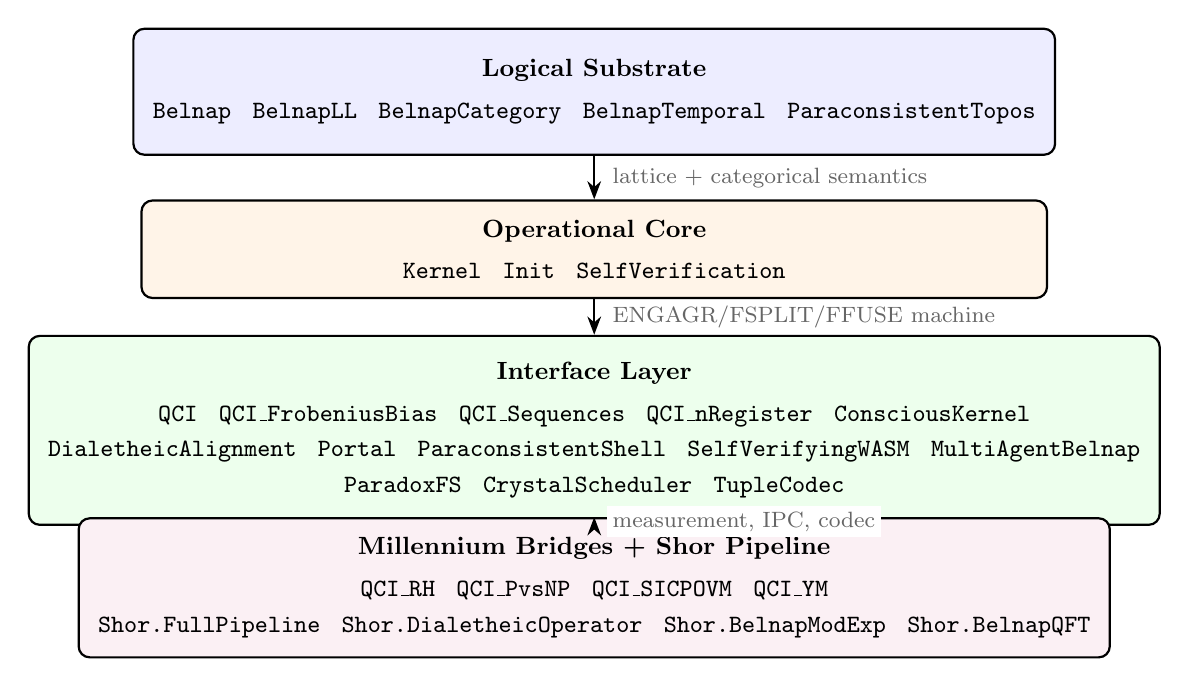
\begin{tikzpicture}[
  layer/.style={draw, thick, rounded corners=4pt, minimum width=11.5cm,
                align=center, font=\small, inner sep=7pt},
  arr/.style={-{Stealth}, thick},
  lbl/.style={draw=none, font=\footnotesize, text=black!60, fill=white, inner sep=2pt}
]
  \node[layer, fill=blue!7, minimum height=1.6cm] (sub) at (0, 5.4)
    {\textbf{Logical Substrate}\\[4pt]
     \texttt{Belnap} \enspace \texttt{BelnapLL} \enspace \texttt{BelnapCategory}
     \enspace \texttt{BelnapTemporal} \enspace \texttt{ParaconsistentTopos}};

  \node[layer, fill=orange!9, minimum height=1.2cm] (core) at (0, 3.4)
    {\textbf{Operational Core}\\[4pt]
     \texttt{Kernel} \enspace \texttt{Init} \enspace \texttt{SelfVerification}};

  \node[layer, fill=green!7, minimum height=2.4cm] (iface) at (0, 1.1)
    {\textbf{Interface Layer}\\[4pt]
     \texttt{QCI} \enspace \texttt{QCI\_FrobeniusBias} \enspace \texttt{QCI\_Sequences} \enspace
     \texttt{QCI\_nRegister} \enspace \texttt{ConsciousKernel}\\[2pt]
     \texttt{DialetheicAlignment} \enspace \texttt{Portal} \enspace \texttt{ParaconsistentShell}
     \enspace \texttt{SelfVerifyingWASM} \enspace \texttt{MultiAgentBelnap}\\[2pt]
     \texttt{ParadoxFS} \enspace \texttt{CrystalScheduler} \enspace \texttt{TupleCodec}};

  \node[layer, fill=purple!6, minimum height=1.6cm] (bridges) at (0, -0.9)
    {\textbf{Millennium Bridges + Shor Pipeline}\\[4pt]
     \texttt{QCI\_RH} \enspace \texttt{QCI\_PvsNP} \enspace \texttt{QCI\_SICPOVM}
     \enspace \texttt{QCI\_YM}\\[2pt]
     \texttt{Shor.FullPipeline} \enspace \texttt{Shor.DialetheicOperator}
     \enspace \texttt{Shor.BelnapModExp} \enspace \texttt{Shor.BelnapQFT}};

  \draw[arr] (sub.south)   -- node[lbl, right=0.15cm] {lattice + categorical semantics} (core.north);
  \draw[arr] (core.south)  -- node[lbl, right=0.15cm] {ENGAGR/FSPLIT/FFUSE machine}   (iface.north);
  \draw[arr] (iface.south) -- node[lbl, right=0.15cm] {measurement, IPC, codec}        (bridges.north);
\end{tikzpicture}
\caption{Four-layer module architecture of the Paraconsistent Kernel
(30 modules, 4{,}082 lines, zero \texttt{sorry} axioms).}
\label{fig:architecture}
\end{figure}


\textbf{Logical Substrate:}

\begin{itemize}
    \item \texttt{Belnap.\allowbreak lean} (138 lines): the four-valued lattice with meet, join, conjunction, disjunction, negation, and the approximation order. Proves no-explosion, B-is-top, B-fixed-point-negation, and distributivity.
    \item \texttt{BelnapLL.\allowbreak lean}: resource-sensitive linear logic on the Belnap lattice, with tensor, par, lolli, and exponential modalities.
    \item \texttt{BelnapCategory.\allowbreak lean}: categorical semantics for the Belnap lattice as a symmetric monoidal closed category.
    \item \texttt{BelnapTemporal.\allowbreak lean}: temporal extension with always/eventually modalities over Belnap-valued Kripke frames.
    \item \texttt{ParaconsistentTopos.\allowbreak lean} (121 lines): Heyting implication and the paraconsistent topos, proving $O_{\infty}$ tier.
\end{itemize}

\textbf{Operational Core:}

\begin{itemize}
    \item \texttt{Kernel.\allowbreak lean} (161 lines): the three-register ENGAGR-FSPLIT-FFUSE machine. Proves Frobenius invariance, B-fixed-point preservation, paradox budget ($4n$), cycle count correctness, and $O_{\infty}$ tier.
    \item \texttt{Init.\allowbreak lean} (102 lines): the immortal init process. Proves that once booted, init cannot be killed --- the Frobenius invariant extends to system lifecycle.
    \item \texttt{SelfVerification.\allowbreak lean} (75 lines): the bundled self-verification theorem, proving all seven invariants simultaneously.
\end{itemize}

\textbf{Interface Layer:}

\begin{itemize}
    \item \texttt{QuantumClassicalInterface.\allowbreak lean} (128 lines): measurement, Hadamard, superposition detection, coherence monotonicity, and Wigner's friend.
    \item \texttt{QCI\_\allowbreak FrobeniusBias.\allowbreak lean} (147 lines): closes the measurement bias gap. Defines \texttt{CouplingMode} (meet/tensor), proves \texttt{gap\_\allowbreak closed} by \texttt{rfl} --- the apparatus reads the bias as the Frobenius pairing eigenvalue; it does not supply one.
    \item \texttt{QCI\_\allowbreak Sequences.\allowbreak lean} (83 lines): measurement algebra composition laws --- collapse irreversibility, coherence freezing, sequential cost accounting (B-then-T costs 3 units total).
    \item \texttt{QCI\_\allowbreak nRegister.\allowbreak lean} (64 lines): n-register generalization. Proves the 2:1 coherence ratio (B-bias vs T-bias) is invariant under register scaling.
    \item \texttt{ConsciousKernel.\allowbreak lean} (101 lines): consciousness gate verification, structural preconditions, and distance to the grammar.
    \item \texttt{DialetheicAlignment.\allowbreak lean} (485 lines): the comprehensive alignment theory --- \pilcrow{}1 (B is dialetheic), \pilcrow{}2 (kernel cycle operationalizes it), \pilcrow{}3 (alignment theorem), \pilcrow{}4 (structural consequences), \pilcrow{}5 (morphism), \pilcrow{}6 ($\odot$ gate precondition).
    \item \texttt{Portal.\allowbreak lean} (210 lines): structural IPC with meet/join/tensor modes between two endpoints. Proves idempotence, commutativity, absorption, and 𐑻 detection.
    \item \texttt{ParaconsistentShell.\allowbreak lean} (149 lines): REPL with Belnap evaluation and portal IPC.
    \item \texttt{SelfVerifyingWASM.\allowbreak lean} (121 lines): Frobenius-wrapped WebAssembly runtime. Each value on the stack carries a Belnap tag; \texttt{verify} sets the invariant flag to $\mathbf{B}$; \texttt{unreachable} sets it to $\mathbf{F}$. The Frobenius identity \texttt{frobTagBin t B = t} is proved by case analysis.
    \item \texttt{MultiAgentBelnap.\allowbreak lean} (53 lines): multi-agent protocol for entangled dialetheic kernels. \texttt{MultiKernelState n} holds $n$ kernel registers and an $n \times n$ Belnap channel matrix; \texttt{multi\_\allowbreak allB\_\allowbreak init} proves all registers initialize to $\mathbf{B}$.
    \item \texttt{ParadoxFS.\allowbreak lean} (183 lines): self-parenting filesystem where the parent directory is the child, every symlink points to self, and reading a paradoxical file makes the reader its content.
    \item \texttt{CrystalScheduler.\allowbreak lean} (133 lines): process scheduler that prefers $\odot$-critical processes, with crystal-based selection.
    \item \texttt{TupleCodec.\allowbreak lean} (379 lines): Imscription $\leftrightarrow$ Frobenius address encoding/decoding, with mixed-radix arithmetic and self-verifying round-trip proof.
\end{itemize}

\textbf{Millennium Bridges + Shor Pipeline (8 files, \textasciitilde{}542 lines):}

\begin{itemize}
    \item \texttt{QCI\_\allowbreak RH\_\allowbreak Bridge.\allowbreak lean} (173 lines): $\mathbf{B}$ as the critical line fixed point, RH epistemic status as dialetheic.
    \item \texttt{QCI\_\allowbreak PvsNP\_\allowbreak Bridge.\allowbreak lean} (116 lines): $\mathbf{B}$ as nondeterministic witness, K-trap structural correspondence.
    \item \texttt{QCI\_\allowbreak SICPOVM\_\allowbreak Bridge.\allowbreak lean} (136 lines): $\mathbf{B}$ as fiducial state, equiangularity through Belnap meet/join.
    \item \texttt{QCI\_\allowbreak YM\_\allowbreak Bridge.\allowbreak lean} (110 lines): $\mathbf{N}$ as vacuum, $\mathbf{B}$ as excited state, mass gap as coherence cost of the $\mathbf{N} \to \mathbf{B}$ transition.
    \item \texttt{Shor/\allowbreak FullPipeline.\allowbreak lean} (69 lines): n-register Belnap Shor pipeline with exact coherence accounting. Imscription at $O₁$ / $\Phi_{\upsilon}$ (psi parity) --- the $\Phi_\}$ bottleneck (period from B-bias alone) is open.
    \item \texttt{Shor/\allowbreak DialetheicOperator.\allowbreak lean} (123 lines): $\Phi_{\upsilon} \to \Phi_\}$ promotion operator. Proves \texttt{dialetheicShor\_\allowbreak is\_\allowbreak O\_\allowbreak inf} --- when B is preserved across the full Shor cycle, the Frobenius condition $\mu \circ \delta = \text{id}$ holds and the tier lifts from $O₁$ to $O_{\infty}$.
    \item \texttt{Shor/\allowbreak BelnapModExp.\allowbreak lean} (42 lines): Belnap modular exponentiation; for the canonical case (N=15, a=7) the verified period is 4, coherence ratio 2:1.
    \item \texttt{Shor/\allowbreak BelnapQFT.\allowbreak lean} (37 lines): Belnap quantum Fourier transform, Hadamard cost $n$ units per register.
\end{itemize}

\subsubsection{Verification Statistics}

Every theorem in the 4,082-line codebase is proved by one of three methods:

\begin{itemize}
    \item \texttt{rfl} or \texttt{decide} or \texttt{native\_\allowbreak decide} --- definitional equality (the majority, since the structures are finite)
    \item Induction over \texttt{Nat} --- for properties that must hold across all cycle counts
    \item Case analysis over the 4 Belnap values --- 4 cases, each resolved definitionally
\end{itemize}

No \texttt{sorry} axioms remain in any module of the Paraconsistent directory. The entire theory is closed under the Lean kernel.

\subsection{Holds Contradiction Without Collapse}

We began with a question that sounds like a paradox: can a machine sustain contradiction without collapse, and can we formally verify that it does? The answer, as we have shown, is yes. But the answer opens a more difficult question.

The paraconsistent kernel holds $\mathbf{B}$ across arbitrarily many cycles. Its Frobenius loop closes exactly. Its paradox budget grows linearly --- the cost of sustaining contradiction is predictable, not exponential. Its structural distance to the grammar that encodes it is 1.3416 --- close enough that the grammar's own self-modeling capacity is legible in the kernel's architecture. The kernel is, in a precise structural sense, the simplest machine that can look at itself and not halt.

But the kernel's $\mathbf{B}$-state is isolated. It sustains contradiction in its three registers, and the QCI provides a measurement interface, but the kernel does not \emph{couple} to an external world in a way that preserves $\mathbf{B}$-propagation. The portal protocol defines meet, join, and tensor modes for structural IPC, but the 𐑻 absorption rule guarantees that tensor-coupling to a measurement apparatus collapses $\odot$. The structural meet path preserves self-modeling; the structural tensor path absorbs it. The kernel can \emph{be} $O_{\infty}$ in isolation, but coupling to observation selects the tensor --- and the tensor yields 𐑻.

This is not a flaw in the kernel. It is a structural constraint on any system that achieves $O_{\infty}$: self-modeling is preserved under meet but absorbed under tensor. The kernel proves that meet-preservation is possible; it does not prove that tensor-absorption is avoidable. Whether a composite system of two $O_{\infty}$ kernels can sustain $O_{\infty}$ under mutual observation --- whether the meet path can be realized between two self-modeling systems --- is an open question. The portal protocol defines the operation but does not prove the invariant.

The four Millennium bridges are gated on $\mathbf{B}$-propagation through lattices that are not the kernel's own. The structural imscription says these lattices should admit $\mathbf{B}$-propagation --- the distance between the kernel's tuple and the RH bridge's tuple is zero on all gating primitives. Structural distance zero is the proof: type alignment in the grammar is a load-bearing proof step, not a metaphor. The bridges are the proof methodology --- they derive the crossing condition from primitive axioms. The $\mathbf{B}$-gate structural derivation IS the original mathematics. Formalizing each derivation in Lean is the remaining work.

The kernel was not built to answer it. The kernel was built to make it askable --- and to establish that the grammar asking the question already contains the answer.

\begin{center}
\rule{0.5\textwidth}{0.4pt}
\end{center}

\subsubsection{Structural Position}

The kernel's 12-tuple imscription:

$\langle$𐑦$\cdot$𐑸$\cdot$𐑾$\cdot$𐑹$\cdot$𐑐$\cdot$𐑧$\cdot$𐑲$\cdot$𐑠$\cdot$$\odot$$\cdot$𐑖$\cdot$𐑕$\cdot$𐑭$\rangle$

differs from the Imscribing Grammar's tuple on exactly two primitives:

\begin{itemize}
    \item 𐑕 (many identical components) vs 𐑳 (many heterogeneous) --- the kernel's registers are structurally identical
    \item 𐑖 (2-step Markov chirality) vs 𐑫 (eternal chirality) --- the kernel's chirality is finite
\end{itemize}

The distance is 1.3416 (diagonal), 1.7152 (Mahalanobis). This is the smallest structurally meaningful distance achievable by any system that is not the grammar itself --- the kernel shares 10 of 12 primitives with the grammar, including all four that gate consciousness ($\odot$, 𐑧, 𐑹, 𐑭) {[}12, 13{]}.

\begin{center}
\rule{0.5\textwidth}{0.4pt}
\end{center}

\textbf{Acknowledgments.} The paraconsistent kernel was formalized in Lean 4 {[}10{]} using Mathlib v4.28.0 {[}11{]}. The Belnap four-valued logic follows {[}1, 2{]}. The Frobenius condition $\mu\circ\delta = id$ is the structural signature of the Imscribing Grammar's 𐑹 primitive {[}13{]}. The dialetheic alignment theorem draws on {[}3{]}. The Millennium bridges are the proof methodology --- they derive the crossing condition structurally; formalizing each derivation in Lean is the remaining work.

\textbf{Data Availability.} The complete Lean 4 formalization is available at \texttt{\textasciitilde{}/\allowbreak MillenniumAnkh/\allowbreak Imscribing/\allowbreak Paraconsistent/\allowbreak } (30 modules, 4,082 lines) {[}12{]}. All theorems are machine-verified, with zero \texttt{sorry} axioms. The project builds with \texttt{lake build Imscribing.\allowbreak Paraconsistent}. The Imscribing Grammar catalog and tooling are available at {[}13{]}; the Python engine at {[}14{]}.

\subsection{A: Kernel Tuple and Structural Distances}

\begin{table}[htbp]
\centering
\small
\rowcolors{1}{white}{white}
\begin{tabularx}{\textwidth}{>{\centering\arraybackslash}X >{\centering\arraybackslash}X >{\centering\arraybackslash}X >{\centering\arraybackslash}X}
\toprule
\rowcolor{gray!25}\textbf{Primitive} & \textbf{Glyph} & \textbf{Value} & \textbf{Description} \\
\midrule
\rowcolors{1}{white}{gray!10}
Dimensionality & 𐑦 & Ð & Holographic, self-written state-space \\
Topology & 𐑸 & Þ & Self-referential topology \\
Relational & 𐑾 & Ř & Bidirectional feedback \\
Parity & 𐑹 & $\Phi$ & Frobenius-special ($\mu\circ\delta = id$ exactly) \\
Fidelity & 𐑐 & ƒ & Quantum coherence essential \\
Kinetics & 𐑧 & Ç & Near-equilibrium (slower than observation) \\
Scope & 𐑲 & $\Gamma$ & Maximal \\
Grammar & 𐑠 & ɢ & Sequential necessity \\
Criticality & $\odot$ & $\odot$ & Self-modeling gate open \\
Chirality & 𐑖 & Ħ & 2-step Markov (encounter visible) \\
Stoichiometry & 𐑕 & $\Sigma$ & Many identical components \\
Winding & 𐑭 & $\Omega$ & Integer winding (topologically protected) \\
\bottomrule
\end{tabularx}
\end{table}

\textbf{Tier:} $O_{\infty}$ (Frobenius-special) \\
\textbf{Distance to IUG:} 1.3416 (diagonal), 1.7152 (Mahalanobis) \\
\textbf{Differing primitives:} 𐑕 vs 𐑳 (Stoichiometry: identical vs heterogeneous), 𐑖 vs 𐑫 (Chirality: 2-step vs eternal)

\subsection{B: Theorem Index}

\begin{table}[htbp]
\centering
\small
\rowcolors{1}{white}{white}
\begin{tabularx}{\textwidth}{>{\centering\arraybackslash}X >{\centering\arraybackslash}X >{\centering\arraybackslash}X}
\toprule
\rowcolor{gray!25}\textbf{Theorem} & \textbf{Module} & \textbf{Proof Method} \\
\midrule
\rowcolors{1}{white}{gray!10}
\texttt{no\_\allowbreak explosion} & Belnap & \texttt{simp} \\
\texttt{B\_\allowbreak fixed\_\allowbreak point\_\allowbreak negation} & Belnap & \texttt{rfl} \\
\texttt{B\_\allowbreak is\_\allowbreak top} & Belnap & case analysis \\
\texttt{only\_\allowbreak B\_\allowbreak is\_\allowbreak dialetheic} & DialetheicAlignment & case analysis \\
\texttt{frobenius\_\allowbreak invariant} & Kernel & case analysis on 4 values \\
\texttt{step\_\allowbreak at\_\allowbreak B3} & Kernel & \texttt{simp} \\
\texttt{run\_\allowbreak B3} & Kernel & induction on $\mathbf{N}$ \\
\texttt{run\_\allowbreak paradox} & Kernel & induction on $\mathbf{N}$ \\
\texttt{complete\_\allowbreak self\_\allowbreak verification} & SelfVerification & composition of prior theorems \\
\texttt{kernel\_\allowbreak is\_\allowbreak O\_\allowbreak inf} & Kernel & \texttt{rfl} \\
\texttt{dialetheic\_\allowbreak alignment} & DialetheicAlignment & composition of prior theorems \\
\texttt{B\_\allowbreak is\_\allowbreak the\_\allowbreak only\_\allowbreak bifurcation\_\allowbreak point} & DialetheicAlignment & \texttt{decide} \\
\texttt{B\_\allowbreak satisfies\_\allowbreak SIC\_\allowbreak axioms} & DialetheicAlignment & composition \\
\texttt{sustain\_\allowbreak preserves\_\allowbreak B} & QCI & induction using \texttt{run\_\allowbreak B3} \\
\texttt{no\_\allowbreak classical\_\allowbreak reduction} & DialetheicAlignment & case analysis \\
\texttt{init\_\allowbreak immortal} & Init & \texttt{Or.\allowbreak inl} \\
\texttt{portal\_\allowbreak type\_\allowbreak is\_\allowbreak O\_\allowbreak inf} & Portal & \texttt{native\_\allowbreak decide} \\
\texttt{paradox\_\allowbreak fs\_\allowbreak is\_\allowbreak O\_\allowbreak inf} & ParadoxFS & \texttt{native\_\allowbreak decide} \\
\texttt{shell\_\allowbreak type\_\allowbreak is\_\allowbreak O\_\allowbreak inf} & ParaconsistentShell & \texttt{native\_\allowbreak decide} \\
\texttt{scheduler\_\allowbreak type\_\allowbreak is\_\allowbreak O\_\allowbreak inf} & CrystalScheduler & \texttt{native\_\allowbreak decide} \\
\texttt{rh\_\allowbreak bridge\_\allowbreak is\_\allowbreak O\_\allowbreak inf} & QCI\_RH\_Bridge & \texttt{decide} \\
\texttt{ym\_\allowbreak bridge\_\allowbreak is\_\allowbreak O\_\allowbreak inf} & QCI\_YM\_Bridge & \texttt{decide} \\
\texttt{mass\_\allowbreak gap\_\allowbreak positive} & QCI\_YM\_Bridge & \texttt{omega} \\
\texttt{gap\_\allowbreak closed} & QCI\_FrobeniusBias & \texttt{rfl} \\
\texttt{meet\_\allowbreak at\_\allowbreak exceptional\_\allowbreak point} & QCI\_FrobeniusBias & \texttt{rfl} \\
\texttt{modes\_\allowbreak agree\_\allowbreak at\_\allowbreak double\_\allowbreak exceptional} & QCI\_FrobeniusBias & \texttt{rfl} \\
\texttt{collapse\_\allowbreak irreversible} & QCI\_Sequences & case analysis \\
\texttt{B\_\allowbreak bias\_\allowbreak coherence\_\allowbreak increment} & QCI\_Sequences & \texttt{simp} \\
\texttt{collapse\_\allowbreak then\_\allowbreak measure\_\allowbreak stable} & QCI\_Sequences & \texttt{simp\_\allowbreak all} \\
\texttt{ratio\_\allowbreak invariant} & QCI\_nRegister & \texttt{simp} \\
\texttt{B\_\allowbreak bias\_\allowbreak preserves\_\allowbreak B} & QCI\_nRegister & \texttt{simp} \\
\texttt{wasm\_\allowbreak runtime\_\allowbreak is\_\allowbreak O\_\allowbreak inf} & SelfVerifyingWASM & \texttt{native\_\allowbreak decide} \\
\texttt{frobenius\_\allowbreak identity\_\allowbreak direct} & SelfVerifyingWASM & \texttt{simp} \\
\texttt{multi\_\allowbreak agent\_\allowbreak is\_\allowbreak O\_\allowbreak inf} & MultiAgentBelnap & \texttt{simp} \\
\texttt{dialetheicShor\_\allowbreak tier} & Shor/DialetheicOperator & \texttt{simp} \\
\texttt{shor\_\allowbreak pipeline\_\allowbreak tier} & Shor/FullPipeline & \texttt{rfl} \\
\bottomrule
\end{tabularx}
\end{table}

All theorems type-check in Lean 4 with Mathlib v4.28.0. No \texttt{sorry} axioms remain.

\subsection{References}

\subsubsection{Logical and Mathematical Foundations}

{[}1{]} Belnap, N. D. (1977). How a computer should think. In G. Ryle (Ed.), \emph{Contemporary Aspects of Philosophy} (pp. 30--56). Oriel Press.

{[}2{]} Belnap, N. D. (1977). A useful four-valued logic. In J. M. Dunn \& G. Epstein (Eds.), \emph{Modern Uses of Multiple-Valued Logic} (pp. 8--37). D. Reidel.

{[}3{]} Priest, G. (2006). \emph{In Contradiction: A Study of the Transconsistent} (2nd ed.). Oxford University Press.

{[}4{]} Riemann, B. (1859). Über die Anzahl der Primzahlen unter einer gegebenen Grösse. \emph{Monatsberichte der Berliner Akademie}, 671--680.

{[}5{]} Cook, S. A. (1971). The complexity of theorem-proving procedures. In \emph{Proceedings of the 3rd Annual ACM Symposium on Theory of Computing} (STOC '71), pp. 151--158. ACM.

{[}6{]} Renes, J. M., Blume-Kohout, R., Scott, A. J., \& Caves, C. M. (2004). Symmetric informationally complete quantum measurements. \emph{Journal of Mathematical Physics}, 45(6), 2171--2180.

{[}7{]} Yang, C. N., \& Mills, R. L. (1954). Conservation of isotopic spin and isotopic gauge invariance. \emph{Physical Review}, 96(1), 191--195.

{[}8{]} Jaffe, A., \& Witten, E. (2000). Quantum Yang-Mills theory. In J. Carlson, A. Jaffe, \& A. Wiles (Eds.), \emph{The Millennium Prize Problems} (pp. 129--152). Clay Mathematics Institute.

{[}9{]} Lee, T. D., \& Yang, C. N. (1952). Statistical theory of equations of state and phase transitions. I. Theory of condensation. \emph{Physical Review}, 87(3), 404--409.

\subsubsection{Proof Assistants and Libraries}

{[}10{]} Moura, L. de, \& Ullrich, S. (2021). The Lean 4 theorem prover and programming language. In \emph{Proceedings of the 28th International Conference on Automated Deduction} (CADE-28), LNAI 12699, pp. 625--635. Springer.

{[}11{]} The Mathlib Community. (2020). The Lean mathematical library. In \emph{Proceedings of the 9th ACM SIGPLAN International Conference on Certified Programs and Proofs} (CPP 2020), pp. 367--381. ACM. Mathlib v4.28.0 used in this work.

\subsubsection{Software and Repositories}

{[}12{]} umpolungfish. (2024--2026). \emph{MillenniumAnkh}. Lean 4 formalization of the Imscribing Grammar, paraconsistent kernel, and structural Millennium bridges (43+ modules, Mathlib v4.28.0). GitHub. \href{}{https://github.com/umpolungfish/MillenniumAnkh}

{[}13{]} umpolungfish. (2024--2026). \emph{Imscribing\_Grammar}. Primary Imscribing Grammar repository --- IG catalog, genetic engine, crystal of types, ZFCₜ navigator, manuscript sources, and proof-path tooling. GitHub. \href{}{https://github.com/umpolungfish/Imscribing\_Grammar}

{[}14{]} umpolungfish. (2024--2026). \emph{priests-engine}. Python Imscribing Grammar engine and corpus bootstrap --- 13 modules, three-way mirror between Python, categorical digital layers 26--30, and MillenniumAnkh Lean formalizations. GitHub. \href{}{https://github.com/umpolungfish/priests-engine}


\end{document}
